\chapter{Theoretical Framework}
\label{sec:theoreticalframework} 

\section{Target Quantification}
\label{sec:dpcr_ch3}

\subsection{Fluorescence, Concentration, and Dilution}
\label{sec:targetconc_ch3_stockDil}
Most molecules are in its state of lowest vibration level at room temperature, and its state becomes excited upon absorbing energy from light. This excitation elevates the molecule to higher vibration levels that cause the emission of fluorescence. The fluorescence intensity of dilute samples is related to physical variables such as the molecular extinction coefficient, quantum efficiency, intensity of incident light \cite{Elmer2000}.

When only a single fluorescent reporter is present, molecules emit only one type of fluorescence intensity. In the process of dPCR, fluorescent probes and primers attach to target sequences in the partitioned reaction mix. When the DNA molecules become excited, each droplet emits a fluorescence endpoint intensity, which is then used to identify if a droplet is positive or negative. An intensity threshold is then determined to classify droplets, such that any intensity less than the threshold is a negative droplet and positive otherwise \cite{Trypsteen2015}. The target concentration is then estimated using the counts of the classified droplets.

In analytical chemistry, the concentration, \(c\), is a measurement of the amount of solute present in an amount of solution,
\[
    c = \frac{\textup{amount of solute}}{\textup{amount of solution}},
\]
\noindent
where the fraction can be in terms of molarity (\(\frac{\textup{moles solute}}{\textup{liters solution}}\)), weight percent (\(\frac{\textup{mL solute}}{\textup{100 mL solution}}\)), weight-to-volume percent (\(\frac{\textup{grams solute}}{\textup{100 mL solution}}\)), etc \cite{Harvey2010}. Unless otherwise stated, concentrations in this paper are in terms of target molecule counts per \(\mu\)L. The concentration formulas specific to dPCR discussed in the following sections are referenced from \citeA{Kreutz2011}, \citeA{Zhu2014}, and \citeA{Gou2018}. 

The dilution factor, \(D\), is the ratio of the initial volume to the final diluted volume (\(V_1 : V_2\)), or equivalently, the ratio of the final diluted concentration to the initial stock concentration (\(c_2 : c_1\)).
\[
    D = \frac{V_1}{V_2} = \frac{c_2}{c_1}
\]

In reporting concentrations, the unknown stock concentration, \(c_1\), is the variable of interest. From the formula above, \(c_1\) can be obtained as 
\begin{equation}
    c_1 = c_2 \times \frac{1}{D}  \label{eq:c1}
\end{equation}

One approach to solve for \(c_1\) is to estimate \(c_2\), the target concentration from the diluted sample. Suppose that the average target copies per droplet  \(\lambda\) is given. Then, a simple unit conversion from \(\lambda\) to \(c_2\) (i.e. from target copies per droplet to target copies per \(\mu\)L) can be derived as follows 
\begin{equation}
    c_2 = \lambda \times \frac{1000}{V_{drp}},  \label{eq:c2}
\end{equation}
\noindent
where \(V_{drp}\) is the known constant droplet volume in terms of nL. Substituting \(c_2\) from equation \ref{eq:c2} to \ref{eq:c1}, and solving for \(\lambda\) brings
\begin{equation}
    \lambda = c_{1} \times \frac{V_{drp}}{1000} \times D, \label{eq:lambda_1}
\end{equation}
\noindent
which will be useful when a dilution series is available as discussed later on Section \ref{sec:targetconc_ch3_loglog}.

\subsection{Poisson Distribution in Counting Target Copies}
\label{sec:targetconc_ch3_poisson}
Let \(X\) be a random variable that represents the number of outcomes that appeared in either a time interval or a region of equal units \(h\) (specified as a time, distance, area, or volume).  \(X\) is defined to follow a Poisson distribution, when the following assumptions are satisfied:

\begin{enumerate}
    \item For all disjoint fixed time intervals or regions, the number of occurences in the span of \(h\) is independent from each other.
    \item The probability of only one outcome happening is proportional to the specified \(h\).
    \item The probability of more than one outcome given a small \(h\) is negligible relative to the probability of only one outcome occuring in the same space.
\end{enumerate}

The probability distribution function of \(X\) is defined as
\[
    P(x; \lambda) = \frac{e^{-\lambda}\lambda^{x}}{x!},\quad x = 0, 1, 2, ...
\]
where \(\lambda\) is the average number of outcomes per fixed time interval or region of \(h\) units \cite{Walpole2011}.

In the context of DNA quantification, the outcome of interest \(X\) is the number of target copies, and the region of fixed sizes \(h\) corresponds to a droplet of equal volumes \(V_{drp}\). The expected value of the target copies \(X\) per droplet, denoted by \(\lambda\) can be estimated using MLE as \(\hat{\lambda} = \frac{1}{n}\sum_{i=1}^{n}x_i\); where \(n\) is the number of independent trials, and \(x_i\) is 1 or 0 for a successful trial. By defining trial as a droplet, and success as a positive droplet, it follows that the probability of getting a positive droplet (i.e. at least one target copy) is \(P(x>0) = \frac{N_{pos}}{N_{tot}}\), where \(N_{tot}\) and \(N_{pos}\) is the count of the total and positive droplets, respectively. The equation below shows how \(\lambda\) can be estimated using Poisson probabilities 
\begin{equation}
    \begin{aligned}
        1-P(x=0) &= P(x>0)\\
        1-e^{-\lambda} &= \frac{N_{pos}}{N_{tot}}\\
        e^{-\lambda} &= 1-\frac{N_{pos}}{N_{tot}}\\
        \hat{\lambda} &= -\ln(1-\frac{N_{pos}}{N_{tot}})\\
        \hat{\lambda} &= -\ln(\frac{N_{neg}}{N_{tot}}) \label{eq:lambda} \\
    \end{aligned}
\end{equation}
Though the last two lines are obviously equivalent, it was derived here since the latter is the commonly used formula for \(\lambda\) \cite{Tzonev2018}. For this study, the comparison between quantification methods will be in terms of \(\hat{\lambda}\) concentration, rather than \(c_{1}\), since the latter is just \(\hat{\lambda}\) multiplied by some constants.

% TODO - Add lambda Confidence Interval formula

\subsection{Log-log Model in Limiting Dilution}
\label{sec:targetconc_ch3_loglog}
Serial dilution assays is a technique to estimate the target concentraton in a population; usually, the dilution factor (a level in the dilution series) progresses in a geometric sequence \cite{Deng2017}. For each dilution factor, sample replicates are prepared; producing a total of \(n\) assays. Let \(D_i\) denote the dilution factor at assay sample \(i\), where \(i={1,2,...,n}\). Then, continuing from equation \ref{eq:lambda_1}, for a given stock conconcentration \(c_1\) diluted by \(D_i\), the expected target copies per droplet is \(\lambda_i\). Thus, it can be said that with a fixed quantity \(c_1\), \(D_i\) is a predictor of \(\lambda_i\). Its relationship in equation \ref{eq:lambda_1} can then be linearized by taking the logarithm on both sides
\begin{equation}
    -\log{(\lambda)} = -\log{(c_1 \times \frac{V_{drp}}{1000})} - \log{(D)} \label{eq:loglambda}
\end{equation}

The proportion of target copies in the droplet population can then be estimated by fitting a binomial generalized linear model (GLM) with a log-log link:
\[
    g(\lambda_i) = \beta_0 + \log{(D_i)}.
\]

In GLM terms, \(\log{D_i}\) is the offset and \(g()\) is the complementary log-log link function resulting in the final model
\begin{equation}
    -\log{(\lambda_i)} = -\log{(c_1 \times \frac{V_{drp}}{1000})} - \log{(D_i)}\beta_1 \label{eq:loglog}
\end{equation}

Equation \ref{eq:loglog} can be formulated as a simple linear regression model \(Y = \beta_0 + X\beta_1 + \epsilon\), where \(\beta_0\) and \(\beta_1\) denotes the slope and intercept, respectively \cite{Walpole2011}. The error term \(\epsilon\) is a random variable assumed to be normally distributed with mean 0 and constant variance \(\sigma^2\). Given a set of ordered pairs {\((x_i,y_i);\) \(i=1,2,...n\)} and an estimated regression model \(\hat{y}_i = b_0 + x_ib_1\), the \(i\)th residual is defined as \(e_i = y_i - \hat{y}_i\). The ordinary least squares (OLS) estimator finds the values of \(b_0\) and \(b_1\) so as to minimize the residual sum of squares
\[
    \textup{SSRes} = \sum_{i=1}^{n}e_i = \sum_{i=1}^{n}(y_i - \hat{y}_i)^2.
\]

The OLS estimates of \(b_0\) and \(b_1\) for the regression coefficients \(\beta_0\) and \(\beta_1\) are 
\[
    b_1 = \frac{\sum_{i=1}^{n}(x_i-\bar{x})(y_i - \bar{y})}{\sum_{i=1}^{n}(x_i-\bar{x})^2}, \quad \textup{and}
\]
\[
    b_0 = \frac{\sum_{i=1}^{n}y_i-b_1\sum_{i=1}^{n}x_i}{n}.
\]

In assay analysis, the interpretation of a slope significantly greater than one implies that the proportion of the target sequence is hyper responsive to the diluted concentration. Otherwise, a slope less than one implies that the proportion of targets is less responsive to the diluted concentration, and suggests heterogeneity.  \cite{Hu2009}.


\section{Evaluation Metrics}
\label{sec:evalmetric_ch3}

\subsection{Precision of Technical Replicates}
\label{sec:evalmetric_ch3_cv}
% TODO : 
% 1. Explain Technical & Biological Variation - [https://www.sigmaaldrich.com/technical-documents/articles/biology/data-analysis.html](https://www.sigmaaldrich.com/technical-documents/articles/biology/data-analysis.html)

In quantitative assay studies, assay variability is typically summarized using the coefficient of variation (CV) \cite{Reed2003}. The CV of \(\hat{\lambda}\) is defined as
\[
    CV = \frac{SD(\hat{\lambda})}{mean(\hat{\lambda})}.
\]

A smaller CV implies good agreement amongst replicate estimates. The advantage of CV over standard deviation (SD) is that it takes into account the magnitude of the units, making CV comparable regardless of analyte concentration.

\subsection{Accuracy of Regression Model}
\label{sec:evalmetric_ch3_R2ResSE}
% TODO : 
% 1. Explain Technical & Biological Variation - [https://www.sigmaaldrich.com/technical-documents/articles/biology/data-analysis.html](https://www.sigmaaldrich.com/technical-documents/articles/biology/data-analysis.html)
% 2. Assuming tehcnical variation only, given a D_i, the expected is lambda_i

Recall that given an estimated regression line, the deviation of the fitted \(\hat{y}\) from the observed \(y\) is the error term \(\epsilon\) with mean 0 and variance \(\sigma^2\). The deviation of \(\epsilon\) measures the model's \emph{lack of fit} \cite{ISLR}. The residual standard error (RSE), or \(\hat{\sigma}\), is the estimated standard deviation of the error terms from fitting a regression model and is calculated as 
\[
    RSE = \sqrt{\frac{1}{n-2}\; \times \textup{SSRes}}.
\]

When the model predicts values that are very close to the observed data, such that \(\hat{y}_i \approx y_i\) for all \(i=1,2,...,n\), then RSE will be very small. On the other hand, predicted values that are far from the actual data will have a large RSE, indicating a poor fit. Since the magnitude of RSE depends on the units of \(Y\), it is not comparable between datasets, and also it is unclear what defines an acceptable RSE. 

In addition to RSE for assessing model accuracy, the coefficient of determination, \(R^2\), is unitless and is in the form of a proportion 
\[
    R^2 = \frac{\textup{SSTotal - SSRes}}{\textup{SSTotal}} = 1-\frac{\textup{SSRes}}{\textup{SSTotal}}.
\]
where \(\textup{SSTotal} = \sum (y_i - \bar{y})^2\) is the total variance in the response \(Y\). Since SSRes is equivalent to the amount of unexplained variance from the regression model, then in contrast, the interpretation of \(R^2\) is the proportion of variability in \(Y\) that can be explained by \(X\). An \(R^2\) close to 1 means that the regressor \(X\) explained a large percentage in the variability in \(Y\), and a value close to 0 means \(X\) does not explain much of the variability in the response.

%These numbers can then be totaled, yielding both a grand total and marginal totals. Totaling the entire table, the number of true positives, false negatives, true negatives, and false positives add up to 100% of the set. Totaling the rows (adding horizontally) the number of true positives and false positives add up to 100% of the test positives, and likewise for negatives. Totaling the columns (adding vertically), the number of true positives and false negatives add up to 100% of the condition positives (conversely for negatives). The basic marginal ratio statistics are obtained by dividing the 2×2=4 values in the table by the marginal totals (either rows or columns), yielding 2 auxiliary 2×2 tables, for a total of 8 ratios. These ratios come in 4 complementary pairs, each pair summing to 1, and so each of these derived 2×2 tables can be summarized as a pair of 2 numbers, together with their complements. Further statistics can be obtained by taking ratios of these ratios, ratios of ratios, or more complicated functions.

\subsection{Binary Classification Metrics}
\label{sec:evalmetric_ch3_binclass}
\begin{figure}[h]
    \centering
    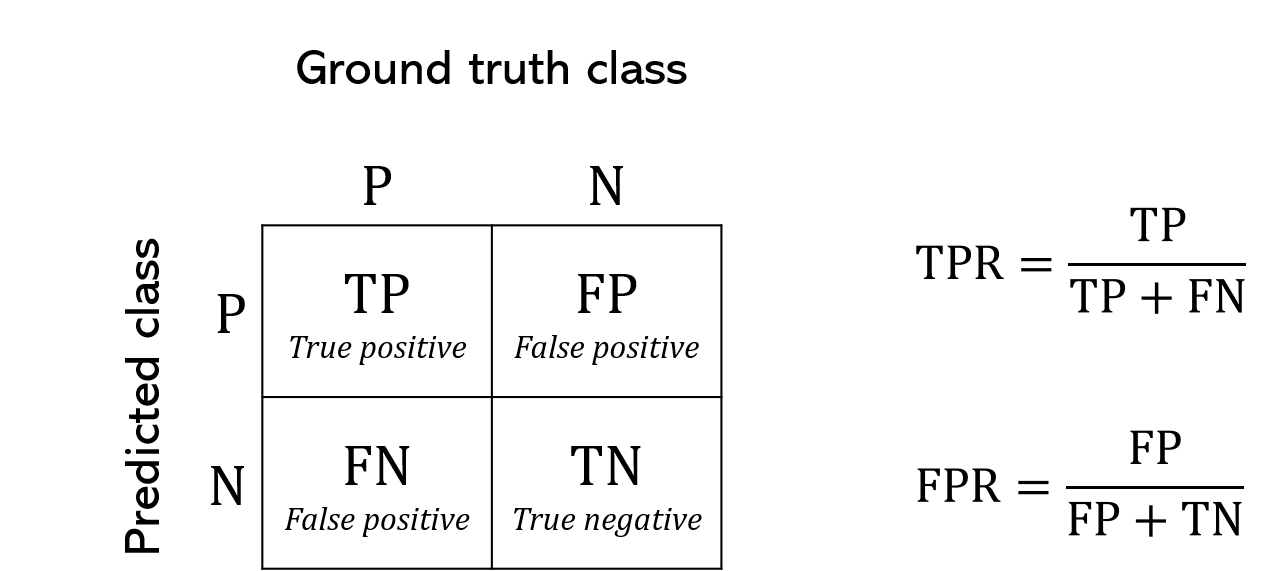
\includegraphics[max size={\textwidth}{\textheight}]{confusionmatrix.png}
    \caption[Confusion matrix with TPR and FPR calculations]{Confusion matrix with TPR and FPR calculations}
        \label{fig:confusionmatrix}
\end{figure}

Most binary classification metrics are founded on the contingency table of ground truth vs predicted conditions, resulting in a tally of the true positives (TP), true negatives (TN), false positives (FP), and false negatives (FN). This table in Figure \ref{fig:confusionmatrix} is also known as the confusion matrix, from which, ratios of cell counts, marginal (row or column) totals, or grand totals can be derived and are used as binary classification metrics. For this study, the classifier metrics False Positive Rate (FPR) and True Positive Rate (TPR) will be assessed. These two statistics are commonly assessed synchronously on a TPR vs FPR plot, called the receiver operating characteristics (ROC) graph. When TPR and FPR pairs are produced from multiple sample sets (or a range of threshold settings), a curve is usually formed in the ROC graph which represents the tradeoff of detection errors (false positives) and benefits (true positives). A good classifier should have more benefits than errors in most cases; that means, in the ROC graph, it is ideal that the points lie very close on the top left corner (1,1), producing a curve that largely covers the graph \cite{Fawcett2006}.
%However, it is not efficient to visually compare ROC curves from several classifiers; what is usually done is to evaluate a single scalar value called the area under the ROC curve (AUC). Since the AUC is bounded by the area of the ROC plot (a unit square), then AUC values fall within 0 to 1.


% Estimated conc as predictor for True conc %
\section{EM Clustering}
\label{sec:modelbased_ch3}

\subsection{G-component Finite Mixture Density}
\label{sec:gcomponentmixturedensity}
Denote \(X=\{x_1, ..., x_N; \myspace x_i \in \mathbb{R}^P\}\) as a statistically independent observation sequence where \(N\) is the number of observations and \(P\) is the dimensionality of \(x_i\), then the G-component finite mixture density is defined as 
\[
    f(X|\theta) = \sum_{g=1}^{G} \pi_g f_g(X|\psi_g),
\]
where \(\pi_g\) is the mixing proportion \((\pi_g > 0, \sum_{g=1}^{G} \pi_g=1\)), \(f_g(X|\psi_g)\) is the \(g\)th component density where \(\psi_g\) are its set of parameters, \(\theta_g \in \theta=\{\theta_1, ..., \theta_G\}\) and \(\theta_g=\{\pi_g,\psi_g\}\) is the unknown parameter set that defines the density function for approximating the true probability of \(X\).


\subsection{Model-based clustering}
\label{sec:modelbasedclustering}
Denote \(C=\{C_1, ..., C_G\}\) as the set of clusters corresponding to each component. \(Z=\{z_1, ..., z_N;\myspace z_i \in C\}\) is the set of ``hidden" states where \(z_i=C_g\) means that the \(g\)th component generated \(x_i\). The indicator variable \(\delta_{gi}\) is introduced to indicate the status of the hidden states as
\[
    \delta_{gi} = \delta(z_i,C_g) = \left\{
        \begin{matrix}
            1 & \textup{ if } x_i \textup{ is generated by cluster } C_g \\ 
            0 & \textup{ otherwise }
        \end{matrix}\right.
\]

Suppose \(X=\{x_1, ..., x_N\}\) of \(N\) \(p\)-dimensional data vectors are observed and all \(N\) are treated as unlabelled. Then the likelihood of a parameter set \(\theta\) given the observed data \(X\) is expressed as 
\begin{equation}
    \begin{array}{l@{} >{\displaystyle}l}
        f(Z,X | \theta)\; & =\prod_{i=1}^{N}f(z_i, x_i | \theta) \\ 
                        & =\prod_{i=1}^{N} \sum_{g=1}^{G} \delta_{gi}f_g(z_i,x_i|\theta_g)\\ 
                        & =\prod_{i=1}^{N} \sum_{g=1}^{G} \delta_{gi}f_g(x_i,z_i=C_g|\theta_g) \\ 
                        & =\prod_{i=1}^{N} \sum_{g=1}^{G}\delta_{gi}f_g(x_i,\delta_{gi}|\theta_g)

    \end{array}
\end{equation}

Suppose that a maximized parameter set \(\theta^*\) has been found. The probability of \(x_i\) belonging to the \(g\)th cluster is defined by the posterior probabilities \(h_g(x_i)=P(\delta_{gi}=1|x_i,\theta^*)\). This can be derived using Bayesian theorem 
\begin{equation}
    \begin{array}{l@{} >{\displaystyle}l}
    h_g(x_i)\;& = P(\delta_{gi}=1|x_i,\theta^*) \\ 
            & = \frac{\pi_gf_g(x_i|\delta_{gi}=1,\psi_g)}{\sum_{k=1}^{G}\pi_kf_k(x_i|\delta_{ki}=1,\psi_k)}\\ 
    \end{array}
\end{equation}

The common method for assigning a cluster \(g\) to \(x_i\) is by using the maximum a posteriori (MAP) classification such that 
\begin{equation}
    \textup{MAP}(\delta_{gi}) = \left\{
        \begin{matrix}
            1 & \textup{ if } \textup{max}_g\{h_g(x_i)\} \textup{ is in cluster } C_g \\ 
            0 & \textup{ otherwise }
        \end{matrix}\right. ,
\end{equation}
\noindent
where \(\textup{MAP}(\delta_{gi})\) of 1 means that amongst all the clusters in \(C\), \(x_i\) has the highest probability to belong to cluster \(C_g\), and is therefore assigned to \(C_g\).

\subsection{Expectation Maximization}
\label{sec:em}
The Expectation-Maximization (EM) algorithm is an approach to finding a maximized likelihood function set \(\theta^*\) for a G-component mixture model. The algorithm starts by guessing the parameter sets, and then iteratively maximizing these parameters using the E-step and M-step until the estimates converge. The EM algorithm are described more in the following :
\begin{enumerate}
    \item \(\mathit{Initialize: }\) Provide an initial guess for the unknown parameter set \(\theta_0\) and set \(t=0\) and \(Q(\theta_0|\theta_{-1})=-\infty\).
    
    \item \(\mathit{E-step: }\) Compute the expected value of the log-likelihood function of \(\theta\) with respect to the current conditional distribution of \(z\) given \(x\) and the current estimates of the parameter \(\theta_t\).
    \begin{equation}        
        \begin{array}{l@{} >{\displaystyle}l}
        Q(\theta|\theta_t) & = E_z[\log{(f(Z,X|\theta))} | X, \theta_t] \\ 
                           & = \prod_{i=1}^{N}\sum_{g=1}^{G}E[\delta_{gi}|x_i,\theta_t] \log(f_g(x_i|\delta_{gi}=1, \psi_g) \pi_g) \\ 
                           & = \prod_{i=1}^{N}\sum_{g=1}^{G}h_{gt}(x_i) \log(f(x_i|\delta_{gi}=1, \psi_g) \pi_g) \\ 
        \end{array}
    \end{equation}
    
    The posterior probability membership function of step \(t\) is computed as
        \begin{equation}
            \displaystyle
            h_{gt}(x_i) = \frac{\pi_{gt}f_g(x_i|\delta_{gi}=1,\psi_{gt})}{\sum_{k=1}^{G}\pi_{kt}f_k(x_i|\delta_{ki}=1,\psi_{kt})}
        \end{equation}

    \item \(\mathit{M-step: }\) Determine the value of \(\theta_{t+1}\) which maximizes \(Q(\theta|\theta_t)\),
    \[
        \theta_{t+1}=\underset{g\epsilon G}{\mathrm{argmax}}{(Q(\theta|\theta_t))}
    \] 
    Deriving this value for the parameter \(\pi_{g,t+1}\) can be done by maximizing \(Q(\theta|\theta_t)\) with respect to \(\pi_{g,t+1}\) by \(\frac{\partial Q(\theta|\theta_t)}{\pi_{gt}}=0\), while subject to the constraint of \(\sum_{g=1}^{G}\pi_g=1\). 
    This finally yields to \(\pi_{g,t+1}=\frac{1}{N}\sum_{i=1}^{N}h_{gt}(x_i)\).

    \item If \(Q(\theta_{t+1}|\theta_{t}) - Q(\theta_{t}|\theta_{t-1}) \le \xi \) (\(\xi \) is the specified termination threshold), then proceed to the last step. Otherwise, go back to Step 2.
    
    \item The final parameter set \(\theta^* = \theta_{t+1}\) is the derived maximized likelihood estimate of \(\theta\).
\end{enumerate}

% \section{EM Parameter Initialization}
% \label{sec:emparaminit_ch3}

% \subsection{Kmeans Clustering}
% \label{sec:kmeans}

% \subsection{Heirarchical Clustering}
% \label{sec:hclust}

% \subsection{Peak Detection}
% \label{sec:peakdetection}

\section{Generalized Hyperbolic Distribution Mixture Models}
\label{sec:ghd_ch3}
The generalized hyperbolic (GH) distribution, first introduced by Barndorff-Nielsen \cite{Barndorff1977}, is a continuous probability distribution with five parameters that describe its location, scale, asymmetry, and the decay of its tails. As the name suggests, this distribution is generalized and is a superclass of the normal inverse Gaussian distributions, scaled t-distributions, standard hyperbolic distributions, variance-gamma distributions, among others. The tails of the GH distribution can range from a Gaussian-like tail to a heavy tail of exponential behavior. Both tails can exhibit different behaviors simultaneously, where the left-hand can be less heavy than the right-hand tail. This property of the GH distribution allows the modeling of asymmetric heavy-tailed populations commonly observed in finance and econometric data \cite{Takahashi2016, Nwobi2014, Necula2009, Aas2006, Bibby2003}. Its applications are in predicting risk models of exchange rates, portfolios, and stock index returns data. 

Let \(X\) be a random variable that follows a generalized hyperbolic distribution with parameters for location (\(\lambda\)), scaling (\(\delta\)), shape (\(\alpha\)), skewness (\(\beta\)), and a parameter \(\mu\) that influences kurtosis and the GH characterization. 
\[
    X \sim GH(\lambda, \alpha, \beta, \delta, \mu)
\]
Then the probability distribution function of \(X\) is defined as
\begin{equation}
    \begin{aligned}[l]
    P(x; \lambda, \alpha, \beta, \delta, \mu) = a(\lambda, \alpha, \beta, \delta, \mu) (\delta^2+(x-\mu)^2)^{1/2\lambda-1/4} \\
    \cdot \; B(\lambda-0.5, \alpha\sqrt{\delta^2+x^2-2x\mu+\mu^2})e^{\beta(x-\mu)}
    \end{aligned}
\end{equation}
where
\[
    a(\lambda, \alpha, \beta, \delta, \mu) = \frac{(\alpha^2-\beta^2)^{1/2\lambda}}{\sqrt{2\pi}\alpha^{\lambda-1/2}\delta^\lambda B(\lambda, \delta\sqrt{\alpha^2 - \beta^2})}
\]
and \(B(\lambda, \cdot)\) denotes the modified Bessel function of the third kind with index \(\lambda\).

GH distribution mixture models were assessed in a study of \citeA{Browne2015} using Old Faithful data \cite{GeyserTimes} and simulated datasets. The former dataset was observed to have skewed tails, and the resulting GH mixture model was shown to have a superior fit as compared to the scale mixture of skew-normal distributions. The simulated dataset was composed of one hundred 2-component mixtures of Gaussian and skew-t distributions. When a GH mixture model was fitted using EM algorithm, all the population parameters were very close to the true values. These demonstrate the ability of GH mixture model to closely capture real data consisting of several populations.